%% Document class
\documentclass[iop,revtex4,numberedappendix,appendixfloats]{emulateapj}

%% General packages
\usepackage{amsmath}
\usepackage{mathrsfs }
\usepackage{lscape}

%% Figure packages
\usepackage{grffile}
\usepackage{subfigure}

%% Referencing
\usepackage{hyperref}

%% Custom macros
\newcommand{\vect}[1]{\boldsymbol{#1}}
\newcommand*\diff{\mathop{}\!\mathrm{d}}
\newcommand*\Diff[1]{\mathop{}\!\mathrm{d^#1}}
\newcommand{\pdf}{\ensuremath{pdf}}
\newcommand{\pmodel}{\ensuremath{p_M}}
\newcommand{\MAP}{MAP}
\newcommand{\MAPs}{MAPs}
\newcommand{\RM}{{\sl RoadMapping}}
\makeatletter
\newcommand{\testlabel}[2]{%
 \protected@write \@auxout {}{\string \newlabel {#1}{{#2}{\thepage}{#2}{#1}{}} }%
 \hypertarget{#1}{#2}
}
\makeatother

\usepackage[usenames,dvipsnames]{xcolor}
\newcommand{\Wilma}[1]{\textcolor{Magenta}{#1}}
\newcommand{\HW}[1]{\textcolor{Green}{#1}}
\newcommand{\Jo}[1]{\textcolor{Blue}{#1}}

%% Abbreviations
\shorttitle{The Influence of Spiral Arms on Action-based Dynamical Modelling of the Milky Way Disk}
\shortauthors{Trick et al.}

\begin{document}

%-----------------------------------------------------------------------------------------------------------------------------------------------------------------------------
%TITLE
%-----------------------------------------------------------------------------------------------------------------------------------------------------------------------------
\title{The Influence of Spiral Arms on Action-based Dynamical Milky Way Disk Modelling\\}

%% Authors
\author{Wilma H. Trick\altaffilmark{1,2}, Jo Bovy\altaffilmark{3}, Elena D'Onghia\HW{???}, and Hans-Walter Rix\altaffilmark{1}}

%% Affiliations
\altaffiltext{1}{Max-Planck-Institut f\"ur Astronomie, K\"onigstuhl 17, D-69117 Heidelberg, Germany}
\altaffiltext{2}{Correspondence should be addressed to trick@mpia.de.}
\altaffiltext{3}{Department of Astronomy and Astrophysics, University of Toronto, 50 St. George Street, Toronto, ON, M5S 3H4, Canada}

%-----------------------------------------------------------------------------------------------------------------------------------------------------------------------------
%ABSTRACT
%-----------------------------------------------------------------------------------------------------------------------------------------------------------------------------

\begin{abstract}
\begin{itemize}
\item One sentence on what RoadMapping is.
\item Overall axisymmetric RoadMapping modelling works in the presence of non-axisymmetric spiral arms, as long as the volume is big enough.
\end{itemize}
\end{abstract}

%-----------------------------------------------------------------------------------------------------------------------------------------------------------------------------
%KEYWORDS
%-----------------------------------------------------------------------------------------------------------------------------------------------------------------------------
\keywords{Galaxy: disk --- Galaxy: fundamental parameters --- Galaxy: kinematics and dynamics --- Galaxy: structure --- \Wilma{[TO DO]}}

%-----------------------------------------------------------------------------------------------------------------------------------------------------------------------------
%INTRODUCTION
%-----------------------------------------------------------------------------------------------------------------------------------------------------------------------------
\section{Introduction}

The first step in learning more about the Milky Way's (MW) overall gravitational potential and orbit distribution function (DF)---which are crucial for understanding galaxy structure and formation---is to find the ``best possible'' axisymmetric model for the Galaxy. Given such a model the identification and characterization of non-axiysmmetries like the bar, spiral arms or stellar streams in stellar phase-space (and chemical abundance) data would then become more straightforward.

Several approaches to constrain an axisymmetric potential and/or orbit DF have recently been put forward: \citet{2013ApJ...779..115B} and \citet{2014MNRAS.445.3133P} fitted potential and DF simultaneously to stellar kinematics in the disk and got precise constraints on the overall potential; \citet{2015MNRAS.449.3479S} and \citet{2016MNRAS.tmp..817D} investigated extended DFs for the disk and halo respectively (given a fiducial potential), that included in addition to the distribution in orbit space also metallicity of the star. 

In this work we will continue our investigation of the \RM{} approach (\emph{``Recovery of the Orbit Action Distribution of Mono-Abundance Populations and Potential INference for our Galaxy''}). The first application of \RM{} was done by \citet{2013ApJ...779..115B} and \citet{Trick 2016}, hereafter Paper I, performed a detailed analysis of the strengths and weaknesses of the approach. 

The idea behind \RM{} is, that simple stellar populations in the MW disk---be it mono-abundance populations \citep{Bovyabcd, ting} \Wilma{TO DO} (i.e., stars with the same $[\mathrm{Fe}/\mathrm{H}]$ and $[\alpha/\mathrm{H}]$ \Wilma{Check}) or maybe also mono-age populations \Wilma{[References: Maybe Martig??? Any Bovy reference about age???]}---follow simple orbit DFs, like, e.g., the quasi-isothermal DF (qDF) by \citet{???}. Given an assumed gravitational potential one can calculate the orbits---or specifically the orbit's actions $\vect{J}=(J_R,J_\phi=L_z,J_z)$, which are integrals of motions---from the star's current phase-space position $(\vect{x},\vect{v})$. Only if the assumed gravitational potential is realistic, this orbital action distribution will follow a realistic orbit DF like the qDF. This allows one to simultaneously fit potential and orbit DF to observations.

\citet{2013ApJ...779..115B} employed this approach to measure the Milky Way's surface density profile within $1.1~\text{kpc}$ using \Wilma{how many?} MAPs in the Galactic disk from the SEGUE survey \Wilma{Check} \Wilma{Reference}. Their potential model had only two \Wilma{Check} free parameters (disk scale length and halo contribution to the radial force at the solar radius). To account for missing model flexibility they constrained the surface density for each MAP only at one best radius. The profile they derived in this fashion had a scale length of $R_s=2.5~\text{kpc}$ and was---in the regime $R>6~\text{kpc}$ \Wilma{Check}---later confirmed by \citet{2014MNRAS.445.3133P} using a different action-based procedure.

Given the success of this first application and in anticipation of the upcoming data releases from Gaia in 2016-2022 \Wilma{Check}, \Wilma{Trick et al. 2016} improved the \RM{} machinery and studied its strengths and breakdowns in detail, by investigating a large suite of mock data sets. Under the prerequisite of axisymmetric data and model, they found that \RM{}'s modelling success is stable against minor misjudgements of DF or selection function, and that---if the true potential is not contained in the proposed family of model potentials---one can still find a good fit, given the limitations of the model. Paper I also found that measurement uncertainties of the order of those by the final Gaia data release should be good enough (within $3~\text{kpc}$ from the Sun) to allow for precise and unbiased modelling results. 

\Wilma{[TO DO: Continue]}

What was not investigated in Paper I, was the breakdown of axisymmetry in the data and what would happen if both axisymmetric distribution function and potential models would therefore not contain the true DF and potential anymore. This will be this work's subject of investigation.

Here we will specifically investigate the important question, if axisymmetric \RM{} modelling can still give reliable constraints on the potential in the presence of non-axisymmetric spiral arms in the data.


\begin{itemize}
\item 
\item Main question: Does axisymmetric RoadMapping modelling work in the presence of non-axiysmmetric spiral arms?
\item Consequences: Both potential and orbit DF are not axisymmetric, i.e., the fitted axisymmetric potential model and DF do per se not contain the truth.
\item How to approach this: Use simulation by D'Onghia et al. 2013 and apply RM to it
\item The potential model we use is chosen mostly for practical reasons and is not necessarily the optimal one for the simulation. Also, we use a single qDF as DF - because it is the simplest thing to do. Also independently of the non-axisymmetries the chosen models might deviate from the truth. Where we investigated deviations between model and truth in isolated test cases, here several assumptions break down simultaneously.
\item Explain actions very shortly. $\vect{J}=(J_R,J_\phi=L_z,J_z)$ quantify oscillation in the coordinate directions $(R,\phi,z)$. Are calculated from current phase-space position in a given potential $\Phi$.
\item Say that actions are conserved in an axisymmetric potential, but not in non-axisymmetric potentials. (Maybe the mean vertical action is conserved \Wilma{[TO DO: Reference]}.) It is therefore important to check, if our modelling works in a system where actions are not conserved.
\end{itemize}

%-----------------------------------------------------------------------------------------------------------------------------------------------------------------------------
%SIMULATION
%-----------------------------------------------------------------------------------------------------------------------------------------------------------------------------
\section{Data from a galaxy simulation} \label{sec:simulation}

%====================
\begin{figure*}[!htbp]
\plotone{fig/plot_simulation_for_paper.pdf}
\caption{Simulation snapshot by \citet{2013ApJ...766...34D} . Shown are the surface mass density (in $(x,y)$ plane, upper panel) and mass density (in $(R,z)$ plane, lower panel) of the ``star'' particles belonging to disk, bulge and giant molecular clouds. (The dark matter halo in this simulation is static and analytic and not shown here.) Overplotted are the disk's scale length $R_s=2.5~\text{kpc}$ (see Section \ref{sec:simulation_description}) and the radii at which we center our test survey volumes in this investigation, $R=8$ and $5~\text{kpc}$. The centers of the different survey volumes are marked with a square, if the survey volume is centered on a spiral arm, or with a circle, if the volume is centerd on an inter-arm region. The yellow circle with radius $r_\text{max}=4~\text{kpc}$ marks the survey volume in which we conduct the analysis discussed in detail in Section \ref{sec:results_part1}. \Wilma{[TO DO: Rename $R_{disk}$ to $R_s$ as it is the scale length of the disk.]} \Wilma{[TO DO: Maybe include spiral arm residuals to show different strength of spiral arms?]}}
\label{fig:simulation}
\end{figure*}
%====================

\subsection{Description of the galaxy simulation} \label{sec:simulation_description}

In this work we use stellar phase-space data drawn from high-resolution N-body simulation snapshot of a disk galaxy by \citet{2013ApJ...766...34D} carried out with GADGET-3 code described in \citet{2005MNRAS.361..776S}, in which overdensities with properties similar to giant molecular clouds induced prominent spiral arms---and therefore non-axisymmetric sub-structure---via the swing amplification mechanism. 

For details see \citet{2013ApJ...766...34D}, here we summarize the essential characteristics.

The simulation has a gravitationally evolving stellar disk within a static/rigid analytic dark matter halo.

The analytic halo follows a \citet{1990ApJ...356..359H} profile
\begin{equation}
\rho_\text{dm}(r) = \frac{M_\text{dm}}{2\pi} \frac{a_\text{dm}}{r (r+a_\text{dm})^3} \label{eq:dm_hernquist}
\end{equation}
with total halo mass $M_\text{dm} = 9.5\cdot 10^{11} ~M_\odot$ and scale length $a_\text{dm} = 29~\text{kpc}$ (Elena D'Onghia, private communication). \HW{[There is no way to check that this is indeed the case. What should I do?]} \Jo{[What does "total mass computed at 160 kpc mean? What does concentration c=9 mean for a Hernquist halo? How does that fit together with a=29 kpc?]}

The disk consists of $10^8$ ``disk star'' particles, each having a mass of $\sim370 ~M_\odot$, and 1000 ``giant molecular cloud'' particles with mass $\sim9.5\cdot 10^{5} ~M_\odot$. Initially the particles are distributed following an exponential disk profile with density
\begin{equation*}
\rho_*(R,z) = \frac{M_*}{4\pi z_0 R_s^2} \text{sech}^2 \left( \frac{z}{z_0}\right) \exp \left(- \frac{R}{R_s} \right),
\end{equation*}
with $R_s = 2.5~\text{kpc}$ and $z_0=0.1R_s$ \Wilma{[TO DO: Check in my own measurements]} and total disk mass $M_* = 0.04\cdot M_\text{dm} = 3.8\cdot 10^{10} M_\odot$ .

The bulge consists of $10^7$ ``bulge star'' particles with mass $\sim950 ~M_\odot$ and they are distributed following a spherical Hernquist profile analogous to Equation \eqref{eq:dm_hernquist}, with total mass $M_\text{bulge}=0.01 \cdot M_\text{dm} = 9.5\cdot 10^9~M_\odot$ and scale length $a_\text{bulge}=0.1\cdot R_s=0.25~\text{kpc}$.

The simulation snapshot which we are using in this work has evolved under its own gravity for $\sim 250~\text{Myr}$, which corresponds to approximately one orbital period at $R\sim8~\text{kpc}$. The mass density of simulation particles (without the DM halo) at this snapshot time is shown in Figure \ref{fig:simulation}. Pronounced spiral arms have developed due to the ``molecular cloud perturbers'', which can be seen in Figure \ref{fig:simulation} as small overdensities in the disk. The spherical bulge and very flattened disk are shown in the lower panel in Figure \ref{fig:simulation}.

We have confirmed that the gravitational center of the particles corresponds to the coordinate origin.

\subsection{Survey volume and data}

The selection function of all-sky surveys like Gaia, that are only limited by the brightness of the tracers, are contiguous and---when ignoring anisotropic effects like dust obscuration---spherical in shape. For simplicity we will use spherical survey volumes centered on different vantage points and with sharp edges at a radius $r_\text{max}$ around it (see also Section \ref{sec:likelihood}), which corresponds to a magnitude cut for stellar tracers all having the same luminosity. Figure \ref{fig:simulation} illustrates the different survey volume positions we use in this study: We use each a volume with $r_\text{max}=1,2,3,4$ or $5~\text{kpc}$ centered on a spiral arm and on an inter-arm region at both the equivalent of the solar radius in this simulation, $R=8~\text{kpc}$, and at $R=5~\text{kpc}$, where the spiral arms are more pronounced (see Figure \Wilma{[TO DO: Make plot that illustrates strengt of spiral arm and reference it here]}) than at $R=~\text{kpc}$. From each volume we draw $N_*=20,000$ random ``disk star'' particles from the simulation and use their phase-space positions $(\vect{x}_i,\vect{v}_i)$ within the simulated galaxy's restframe as data. To make the data sample more realistic, one would actually have to add measurement uncertainties, especially to the distances of the survey volumes central vantage point and the proper motions measured from there. We decided not to include measurement uncertainties: Firstly, their effect on \RM{} modelling has been already investigated in Paper I and we found that the measurement uncertainties of the last data release of Gaia should be small enough to not disturb the modelling to much. Secondly, in this study we want to isolate and investigate the deviations of the data from the assumed potential and DF model and axisymmetry independently of other effect.

\subsection{Symmetrized potential model}

For a galaxy with pronounced spiral arms an axisymmetric model matter distribution can per se not reproduce the truth. However, there should be a ``best possible'' symmetric model for the galaxy, which would then be by construction the best we can do with RoadMapping. We derive therefore a ``true symmetrized'' potential model directly from the snapshot via two different methods: One based on the density distribution of the different galaxy components, and the other based on the known true gravitational potential at the position of the stars. 

The first approach uses our previous knowledge about the bulge and halo, which follow both a Hernquist profile with well-defined parameters by construction (see Section \Wilma{???}). The disk with its spiral arms however does deviate strongly from its initial conditions in Equation \Wilma{???}. We use two different disk models available in the \texttt{galpy} (galaxy python) library, the double exponential disk and the Miyamoto-Nagai disk, and fit them to the overall density distribution of the snapshots disk particles. The parameters of the two best fit potential models, the \texttt{DEHH-Pot} (Double Exponential disk, Hernquist halo, Hernquist bulge) and \texttt{MNHH-Pot} (Miyamoto-Nagai disk, Hernquist halo, Hernquist bulge), are given in Table \ref{tbl:symmetrizedpotential}.

The second approach uses the exact same potential as the \RM{} machinery (see Section \Wilma{???}): A potential of the same shape as \texttt{MNHH-Pot}, with fixed and known bulge, but unknown disk and halo parameters. The simulation snapshot provides the local true potential evaluated at the position of each star. We pick 1 million random disk particles (to speed up the fitting) within $R=2-14~\text{kpc}$ and then run a MCMC that fits this \texttt{MNHH-Pot} to the true local potential at the given stellar positions. The resulting parameters and uncertainties are given in Table \ref{tbl:symmetrizedpotential} as well. The uncertainties are relatively large, especially in the disk scale height, because (a) the local true potential varies strongly with the the spiral arms and (b) the fitted potential model has no previous knowledge about the contribution of disk and halo relative to each other as the first approach. Also, most of the stars are located in the plane of the disk and in spiral arms, which might bias the result. 

In any case, these models give a benchmark, what we can maximally expect to achieve with \RM{}.

%====================
\begin{deluxetable*}{llllll}[!htbp]
\tabletypesize{\scriptsize}
\tablecaption{??? \label{tbl:symmetrizedpotential}}
\tablewidth{0pt}
\tablehead{
\colhead{potential model} & \colhead{circular velocity} & \colhead{disk scale lentgh} & \colhead{disk scale height} & \colhead{halo fraction} & \colhead{halo scale length} \\
 &  \colhead{$v_\text{circ}(R_\odot)$ [km s$^{-1}$]} & \colhead{[kpc]} & \colhead{[kpc]} & \colhead{$f_\text{halo}$} & \colhead{$a_\text{halo}$ [kpc]}}
\startdata
\texttt{DEHH-Pot} (from disk density) & $222$ & $h_r: 2.5$ & $h_z: 0.17$ & $0.54$ & $29$\\
\texttt{MNHH-Pot} (from disk density) & $215$ & $a_\text{disk}: 2.35$ & $b_\text{disk}: 0.21$ & $0.57$ & $29$\\
\texttt{MNHH-Pot} (from snapshot potential) & $225_{-1}^{+1}$ & $a_\text{disk}: 3.1_{-1.3}^{+0.5}$ & $b_\text{disk}: 0.4_{-0.3}^{+1.3}$ & $0.57_{-0.08}^{+0.09}$ & $25_{-3}^{+4}$\\
\enddata
%\tablenotetext{(a)}{...}
\end{deluxetable*}
%====================

\subsection{Quantifying influence of spiral arm}

\Wilma{[TO DO: There is a short comment on that in D'Onghia 2013 as well]}

Depending on size and position of the survey volume the spiral arms and inter-arm regions dominate the stellar distribution within the survey volume to different degrees. To quantify the strength of the spiral arm, we introduce the quantity
\begin{equation*}
\kappa(x_j,y_j) \equiv \frac{\Sigma_{\text{disk},T}(x_j,y_j \mid z\leq z_j)}{\Sigma_{\text{disk},S}(x_j,y_j \mid z\leq z_j)} -1
\end{equation*}
where $\Sigma_{\text{disk},i}$ is the surface density of the disk component  of the simulation snapshot ($i=T$) or of the symmetrized snapshot model in Section \Wilma{[TO DO]} ($i=S$) within the survey volume,
\begin{eqnarray*}
\Sigma_{\text{disk},i} &\equiv& \int_{-z_j}^{z_j} \rho_{\text{disk},i}(x_j,y_j,z) \ \diff z\\
z_j &=& \begin{cases}
\sqrt{r_\text{max}^2 - (x_j-x_c)^2 - (y_j-y_c)^2} & \text{for sf}(x_j,y_j,0) > 0\\
0 & \text{otherwise.}
\end{cases}
\end{eqnarray*}
$(x_c,y_c,z_c=0)$ is the position of the survey volume's center within the simulation's cartesian coordinate system. $(x_j,y_j)$ is the centroid of a surface area element $(x_j\pm\delta,y_j\pm \delta)$ with $\delta=\Wilma{???}$. We calculate $\kappa(x_j,y_j)$ for all $n \simeq \pi r_\text{max}^2/4\delta^2$ surface elements within the survey volume. The statistics
\begin{eqnarray*}
\langle \kappa \rangle &\equiv& \frac 1n \sum_j^n \kappa(x_j,y_j)\\
\sigma_\kappa &\equiv& \sqrt{\frac 1n \sum_j^n \left(\kappa(x_j,y_j) - \langle \kappa \rangle \right)^2}
\end{eqnarray*}
give us information if a single spiral arm or an inter-arm region dominates the survey volume ($\langle \kappa \rangle$ large for spiral arms, $\langle \kappa \rangle$ small for inter-arm regions, at small $\sigma_\kappa$) or if several spiral arms cross the survey volume (large $\sigma_\kappa$).

\Wilma{[TO DO: Test also alternative models, i.e., a) using the intial condition disk density within the surface density, b) ignoring the z-height and using the best fit surface density with scale length 2.5kpc.]}

%-----------------------------------------------------------------------------------------------------------------------------------------------------------------------------
%MODELLING
%-----------------------------------------------------------------------------------------------------------------------------------------------------------------------------
\section{RoadMapping modelling}

\subsection{Likelihood} \label{sec:likelihood}

The data that goes into the modelling are the 6D position and velocity coordinates $(\vect{x}_i,\vect{v}_i)$ of $N_*$ stars within the survey volume. For simplicity we use a purely spatial selection function $\text{sf}(\vect{x})$ of spherical shape,
\begin{equation*}
\text{sf}(\vect{x}) \equiv \begin{cases} 1 &\mbox{if } \left| \vect{x}-\vect{x}_0 \right| \leq r_\text{max} \\
0 & \mbox{otherwise} \end{cases},
\end{equation*}
whose maximum radius $r_\text{max}$ defines the boundary of the survey volume and which is centred on $\vect{x}_0 \equiv (R_0,\phi_0,z_0=0)$. Given a parametrized potential model $\Phi(R,z)$ with parameters $p_\Phi$, the $i$-th star is on an orbit characterized by the orbital actions 
\begin{equation*}
\vect{J}_i \equiv \vect{J}[\vect{x}_i,\vect{v}_i \mid p_\Phi].
\end{equation*}
The probability of stars to be on the orbit $\vect{J}_i$ is proportional to a given orbit distribution function $\text{df}(\vect{J})$ with parameters $p_\text{DF}$,
\begin{equation*}
\text{df}(\vect{J}_i \mid p_\text{DF}) \equiv \text{df}(\vect{J}[\vect{x}_i,\vect{v}_i \mid p_\Phi] \mid p_\text{DF}) \equiv \text{df}(\vect{x}_i,\vect{v}_i \mid p_\Phi,p_\text{DF}),
\end{equation*} 
where the latter equivalence arises from the Jacobian determinant between the angle-action coordinates $(\vect{\theta},\vect{J})$ and cartesian phase-space coordinates $(\vect{x},\vect{v})$, which is $\left| \partial (\vect{x},\vect{v}) / \partial(\vect{\theta},\vect{J})\right|=1$ and therefore allows us to treat the $\text{df}$ equivalently as a distribution of current phase-space coordinates or a distribution of orbital actions only, with uniform distribution in the angles $\vect{\theta}$. In some sense, the $\text{df}(\vect{J})$ describes how we expect a realistic stellar population in the MW disk to look like.

The joint likelihood of the $i$-th star being on an orbit $\vect{J}$ in the potential $\Phi$ and being within the survey volume is therefore
\begin{equation*}
\mathscr{L}_i \equiv \mathscr{L}(\vect{x}_i,\vect{v}_i) = \frac{\text{df}(\vect{x}_i,\vect{v}_i\mid p_\phi, p_\text{DF}) \cdot \text{sf}(\vect{x_i})}{\int \text{df}(\vect{x},\vect{v}\mid p_\Phi, p_\text{DF}) \cdot \text{sf}(\vect{x}) \ \Diff3 x \Diff3 v}.
\end{equation*}
The details how we evaluate the likelihood normalisation numerically to sufficiently high enough precision are discussed in Paper I.\footnote{\Wilma{[TO DO: Write what exact numerical accuracy we use and check that it is actually good enough.]}}

In the scenario considered in this paper it can happen that there are a few ($\sim 1$ in 20,000) stars entering the catalogue that are for some reason  on rather extreme orbits, e.g., moving radially directly towards the center. These kinds of orbits do not belong to the set of orbits that we classically expect to make up a overall smooth galactic disk. To avoid that such single stars with very low likelihood mess up the modelling we introduce here a simple outlier model,
\begin{equation*}
\mathscr{L}_i \longrightarrow \max \left( \mathscr{L}_i, \epsilon \cdot \text{median}(\mathscr{L})\right),
\end{equation*}
where $\epsilon = 0.001$ for $N_*=20,000$ stars and $\text{median}(\mathscr{L})$ is the median of all the $N_*$ stellar likelihoods $\mathscr{L}_i$ with the given $p_\Phi$ and $p_\text{DF}$. This outlier model was not used in Paper I.

Following Paper I, we assume for now uninformative flat priors on the model parameters $p_\Phi$ and $p_\text{DF}$ and find the maximum and width of the posterior probability function
\begin{equation*}
pdf(p_\Phi,p_\text{DF} \mid \text{data}) \propto \prod_{i=1}^{N_*} \mathscr{L}_i \cdot prior(p_\Phi,p_\text{DF})
\end{equation*}
using a nested-grid approach and then explore the full shape of the $\pdf$ using a Monte Carlo Markov Chain (MCMC)\footnote{\Wilma{[TO DO: Reference emcee]}}. Full details on this procedure are given in Paper I.

\subsection{DF model}

The most simple orbit distribution function exhibiting a disk-like structure may be the quasi-isothermal distribution function (qDF) introduced by \citet{2010MNRAS.401.2318B} and \citet{2011MNRAS.413.1889B}. It  proofed to be a successful model to describe the orbit distribution of individual mono-abundance populations (MAPs) in the Galactic disk \citep{2013ApJ...779..115B,2013MNRAS.434..652T}, that seem to be isothermal in $z$-direction (i.e., ``quasi-isothermal''). Modelling approaches trying to capture the overall disk distribution \citep{2014MNRAS.445.3133P,2015MNRAS.449.3479S} were describing the Galactic disk as a superposition of many qDFs. The qDF, which we already used in Paper I, has the functional form
\begin{eqnarray}
&&\text{qDF}(\vect{J} \mid p_\text{DF}) \nonumber\\
&&= f_{\sigma_R}\left(J_R,L_z \mid p_\text{DF}\right) \times f_{\sigma_z}\left(J_z,L_z \mid p_\text{DF}\right)\label{eq:df_general}\end{eqnarray}
where
\begin{eqnarray}
f_{\sigma_R}\left(J_R,L_z \mid p_\text{DF}\right) &=& n \times \frac{\Omega}{\pi\sigma_R^2(R_g) \kappa}\exp\left(-\frac{\kappa J_R}{\sigma_R^2(R_g)} \right) \nonumber\\
&& \times \left[1+\tanh\left(L_z/L_0\right) \right]\\
f_{\sigma_z}\left(J_z,L_z \mid p_\text{DF} \right) &=& \frac{\nu}{2 \pi \sigma_z^2(R_g)} \exp\left( -\frac{\nu J_z}{\sigma_z^2(R_g)} \right)
\end{eqnarray}
\citep{2011MNRAS.413.1889B}. The guiding-center radius $R_g$, circular frequency $\Omega$, radial/epicycle frequency $\kappa$ and vertical frequency $\nu$ describe the near-circular orbit with given angular momentum $L_z$ in a given potential. Counter-rotating orbits with $L_z < L_0$ are suppressed by the term $\left[1+\tanh\left(L_z/L_0\right) \right]$ (with $L_0 \sim 10~\text{km s}^{-1}~ \text{kpc}$). 
We set the radial stellar tracer density $n(R_g)$ and velocity dispersion profiles $\sigma_z(R_g)$ and $\sigma_R(R_g)$ to
\begin{eqnarray}
n(R_g \mid p_\text{DF}) &\propto& \exp\left(-\frac{R_g}{h_R} \right)\\
\sigma_R(R_g \mid p_\text{DF}) &=& \sigma_{R,0} \times \exp\left(- \frac{R_g-R_\odot}{h_{\sigma,R}} \right)\label{eq:sigmaRRg}\\
\sigma_z(R_g \mid p_\text{DF}) &=& \sigma_{z,0} \times \exp\left(- \frac{R_g-R_\odot}{h_{\sigma,z}} \right)\label{eq:sigmazRg}.
\end{eqnarray}
The free model parameters of the qDF are therefore
\begin{equation*}
p_\text{DF} \equiv \left\{ \ln h_R, \ln \sigma_{R,0}, \ln \sigma_{z,0}, h_{\sigma,R}, h_{\sigma,z}\right\}.
\end{equation*}

Even though we do not have any stellar abundance or age information in the simulation snapshot we are going to investigate (see Section \ref{sec:simulation}) and we therefore cannot define stellar sub-populations for which the assumption of such a simple model might be reasonable, we will still try to model the whole disk with a single qDF---to see how far we can get with the simplest possible model.

\subsection{Potential model}

\Wilma{[TO DO]}

\begin{itemize}
\item Introduce potential model, explain that form of disk was mostly chosen to the closed form expression of $Phi$ which allows for fast calculation. Both MNHH, DEHH and KKS pot.
\item Mention action calculation and that we tested explicitely that fixing Delta=0.45 and using staeckel interpolation grid does not degrade the analysis
\item \Wilma{Mention and reference galpy.}
\end{itemize}

%-----------------------------------------------------------------------------------------------------------------------------------------------------------------------------
%RESULTS
%-----------------------------------------------------------------------------------------------------------------------------------------------------------------------------
\section{Results}

\subsection{A single application of \RM{}} \label{sec:results_part1}

In this section we will discuss the results of the \RM{} analysis of a single data set. This fiducial data set has $N_*=20,000$ stars that were drawn from the spherical volume with $r_\text{max}=4~\text{kpc}$ centered on a spiral arm at the ``solar'' radius $R=8~\text{kpc}$ shown as yellow sphere in Figure \ref{fig:simulation}. We use \RM{} to fit a single qDF (see Section \Wilma{[TO DO]}) and the potential model consisting of a Miyamoto-Nagai disk, a Hernquist halo and a (fixed) Hernquist bulge introduced in Section \Wilma{[TO DO]} to it.

\subsubsection{Recovering the stellar distribution}

\begin{itemize}
\item Figure: (x,y) and (R,z) distribution of residuals of true and best fit stellar distribution. Mark spiral arms as circles with radius Rg.
\item Figure: 1D histograms in R,z,phi, comparison of  true, best fit and best fit in symmetrized potential
\item Figure: 1D histograms in velocity and different (R,z,phi) bins comparison of  true, best fit and best fit in symmetrized potential
\end{itemize}

%====================
\begin{figure*}[!htbp]
  \centering
  \begin{subfigure}
    \centering
    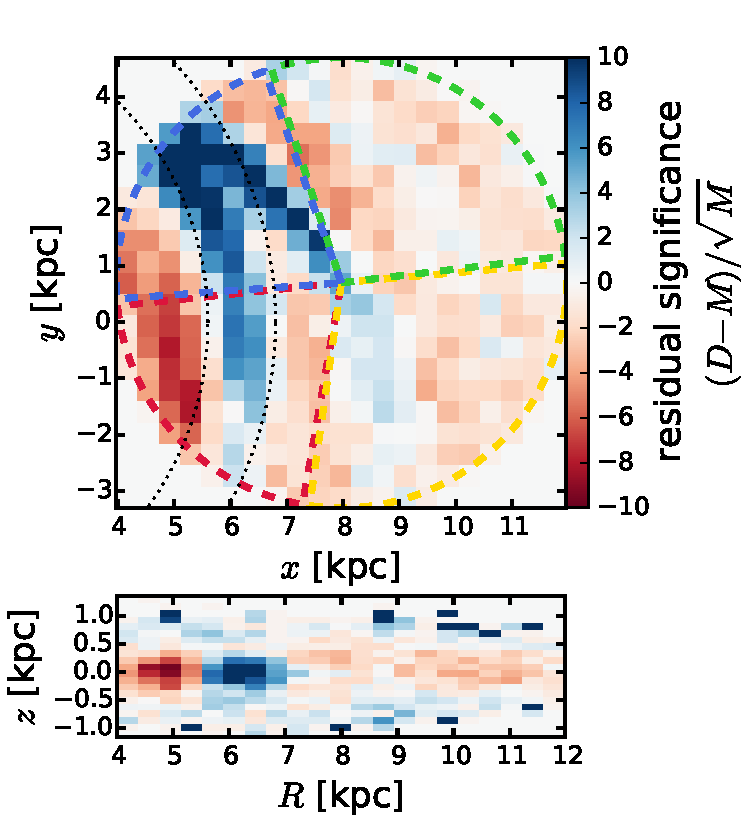
\includegraphics[width=.3\linewidth]{fig/MNdHHdiffSph2_4kpc8Spiral_a_test1_data_bestfit_residuals_3a.pdf}
    \caption{Caption 1}
    \label{fig:???}
  \end{subfigure}%
  \quad
  \begin{subfigure}
    \centering
    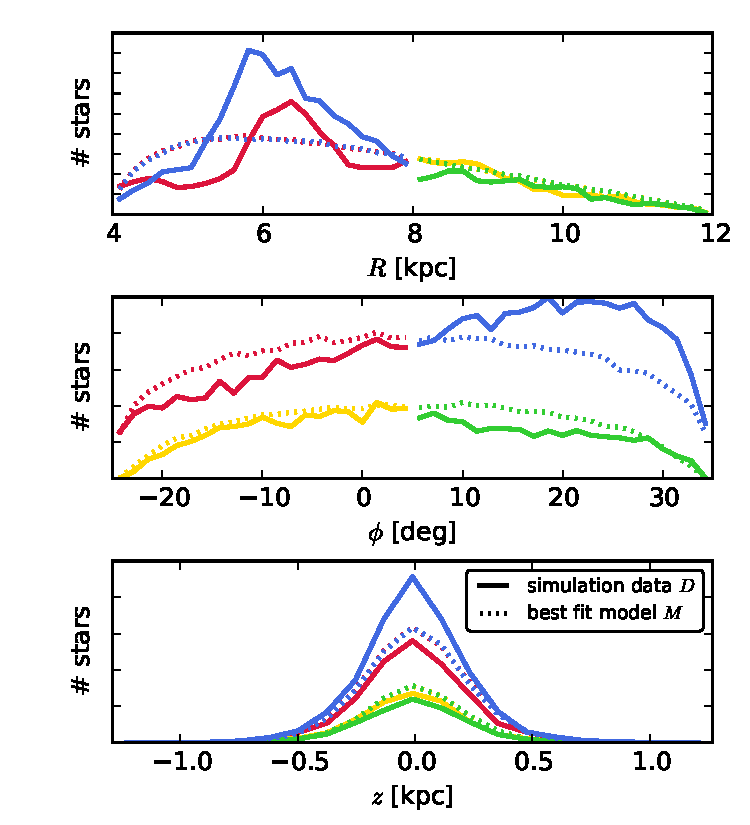
\includegraphics[width=.3\linewidth]{fig/MNdHHdiffSph2_4kpc8Spiral_a_test1_data_bestfit_residuals_3b.pdf}
    \caption{Caption 2}
    \label{fig:???}
  \end{subfigure}%
  \quad
  \begin{subfigure}
    \centering
    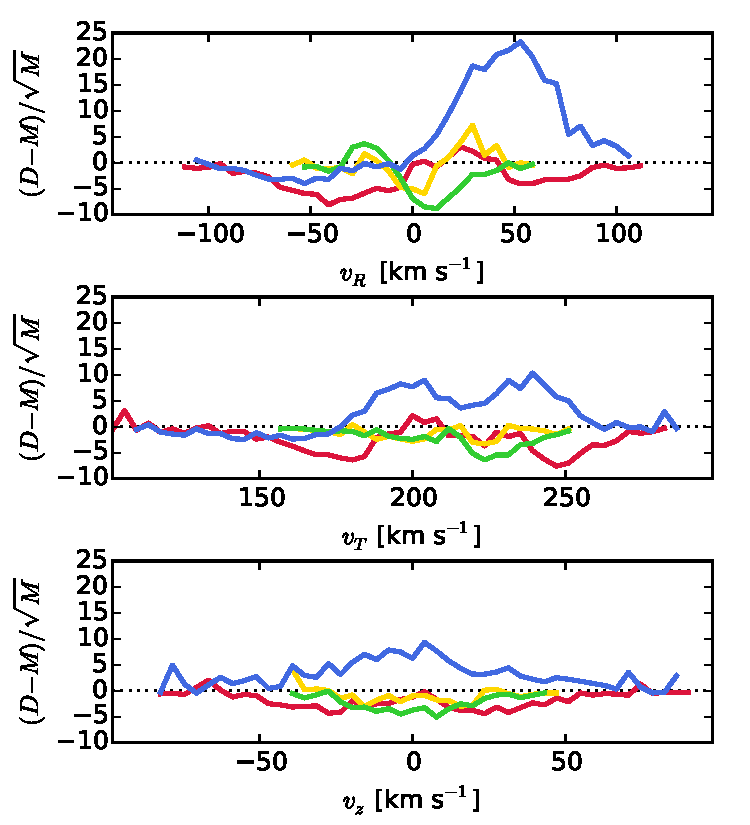
\includegraphics[width=.3\linewidth]{fig/MNdHHdiffSph2_4kpc8Spiral_a_test1_data_bestfit_residuals_3c.pdf}
    \caption{Caption 2}
    \label{fig:???}
  \end{subfigure}
  \caption{Side-by-side figures.}
  \label{fig:???}
\end{figure*}
%====================


\subsubsection{Recovering the potential}

Figures \Wilma{[TO DO]} demonstrate the recovery of the simulation's gravitational potential with \RM{}. Figure \Wilma{[TO DO]} compares the true density distribution with the density distribution of the symmetrized simulation potential in Section \Wilma{[TO DO]} and the recovered \RM{} density distribution. \Wilma{[TO DO]}

%====================
\begin{figure*}[!htbp]
\plotone{fig/MNdHHdiffSph2_4kpc8Spiral_a_test1_density_overview.pdf}
\caption{Comparison of the true density distribution $\rho_{\Phi,\text{T}}$ in the galaxy simulation snapshot (solid black line, averaged over $\phi$) with the axisymmetric density distribution $\rho_{\Phi,\text{R}}$ recovered with \RM{} (solid blue lines) from $N_*=20,000$ stars in the survey volume with $r_\text{max}=4~\text{kpc}$ (yellow line), as described in Section \Wilma{[TO DO]}. The first two panels show density profiles along $(R,z=0)$ and $(R=8~\text{kpc},z)$, together with the relative differences between true and recovered $\rho_{\Phi}$. The third panel displays equidensity contours of the matter distribution in the $(R,z)$ plane. Overplotted are also the symmetrized ''true´´ potential's $\rho_{\Phi,\text{S}}$ (dotted black line) (see Section \Wilma{[TO DO]}) and the $\rho_{\Phi,\text{M}}$ of the recovered mean model in Table \Wilma{[TO DO]} (dotted blue line). The last panel shows the relative difference between the true $\rho_{\Phi,\text{T}}$ (averaged over all $\phi$) and the recovered mean model $\rho_{\Phi,\text{M}}$. Over wide areas even outside of the survey volume the relative difference is less than $15\%$. At $R\gtrsim8~\text{kpc}$ and $z\sim0$ it becomes apparent that the chosen potential model cannot perfectly capture the structure of the disk. \Wilma{[TO DO: Make sure that this plot actually contains the final analysis and sym. model that I want to show.]} \Wilma{[TO DO: Maybe it would be more interesting to see a best fit MNd directly to the potential to see, how well the potential model can actually perform?]} \Wilma{[TO DO: Maybe use only stars in the cone that the survey volume probes???]}}
\label{fig:???}
\end{figure*}
%====================

%====================
\begin{figure*}[!htbp]
\plotone{fig/MNdHHdiffSph2_4kpc8Spiral_a_test1_vcirc_surfdens_overview.pdf}
\caption{Comparison of the circular velocity curve, surface density profile within $|z|\leq1.1~\text{kpc}$ and disk-to-halo ratio of the surface density along $R$ for the true potential of the galaxy simulation snapshot (solid black line) and the axisymmetric model potential recovered with \RM{} (solid blue lines) (see Section \Wilma{[TO DO]}). Overplotted are also the profiles of the symmetrized ''true´´ potential (dotted black line) (see Section \Wilma{[TO DO]}) and the recovered mean model (dotted blue line) (see Table \Wilma{[TO DO]}). The circular velocity curve is recovered to less than $5\%$, especially at larger radii. For the surface density and disk-to-halo ratio \RM{} recovers the truth at radii $\lesssim 8~\text{kpc}$. The deviations at larger radii are connected to the discrepancies in the density in Figure \Wilma{[TO DO]}. \Wilma{[TO DO: When I have the force I can probably also calculate the true circular velocity curve!]}}
\label{fig:???}
\end{figure*}
%====================

%====================
\begin{figure*}[!htbp]
\centering
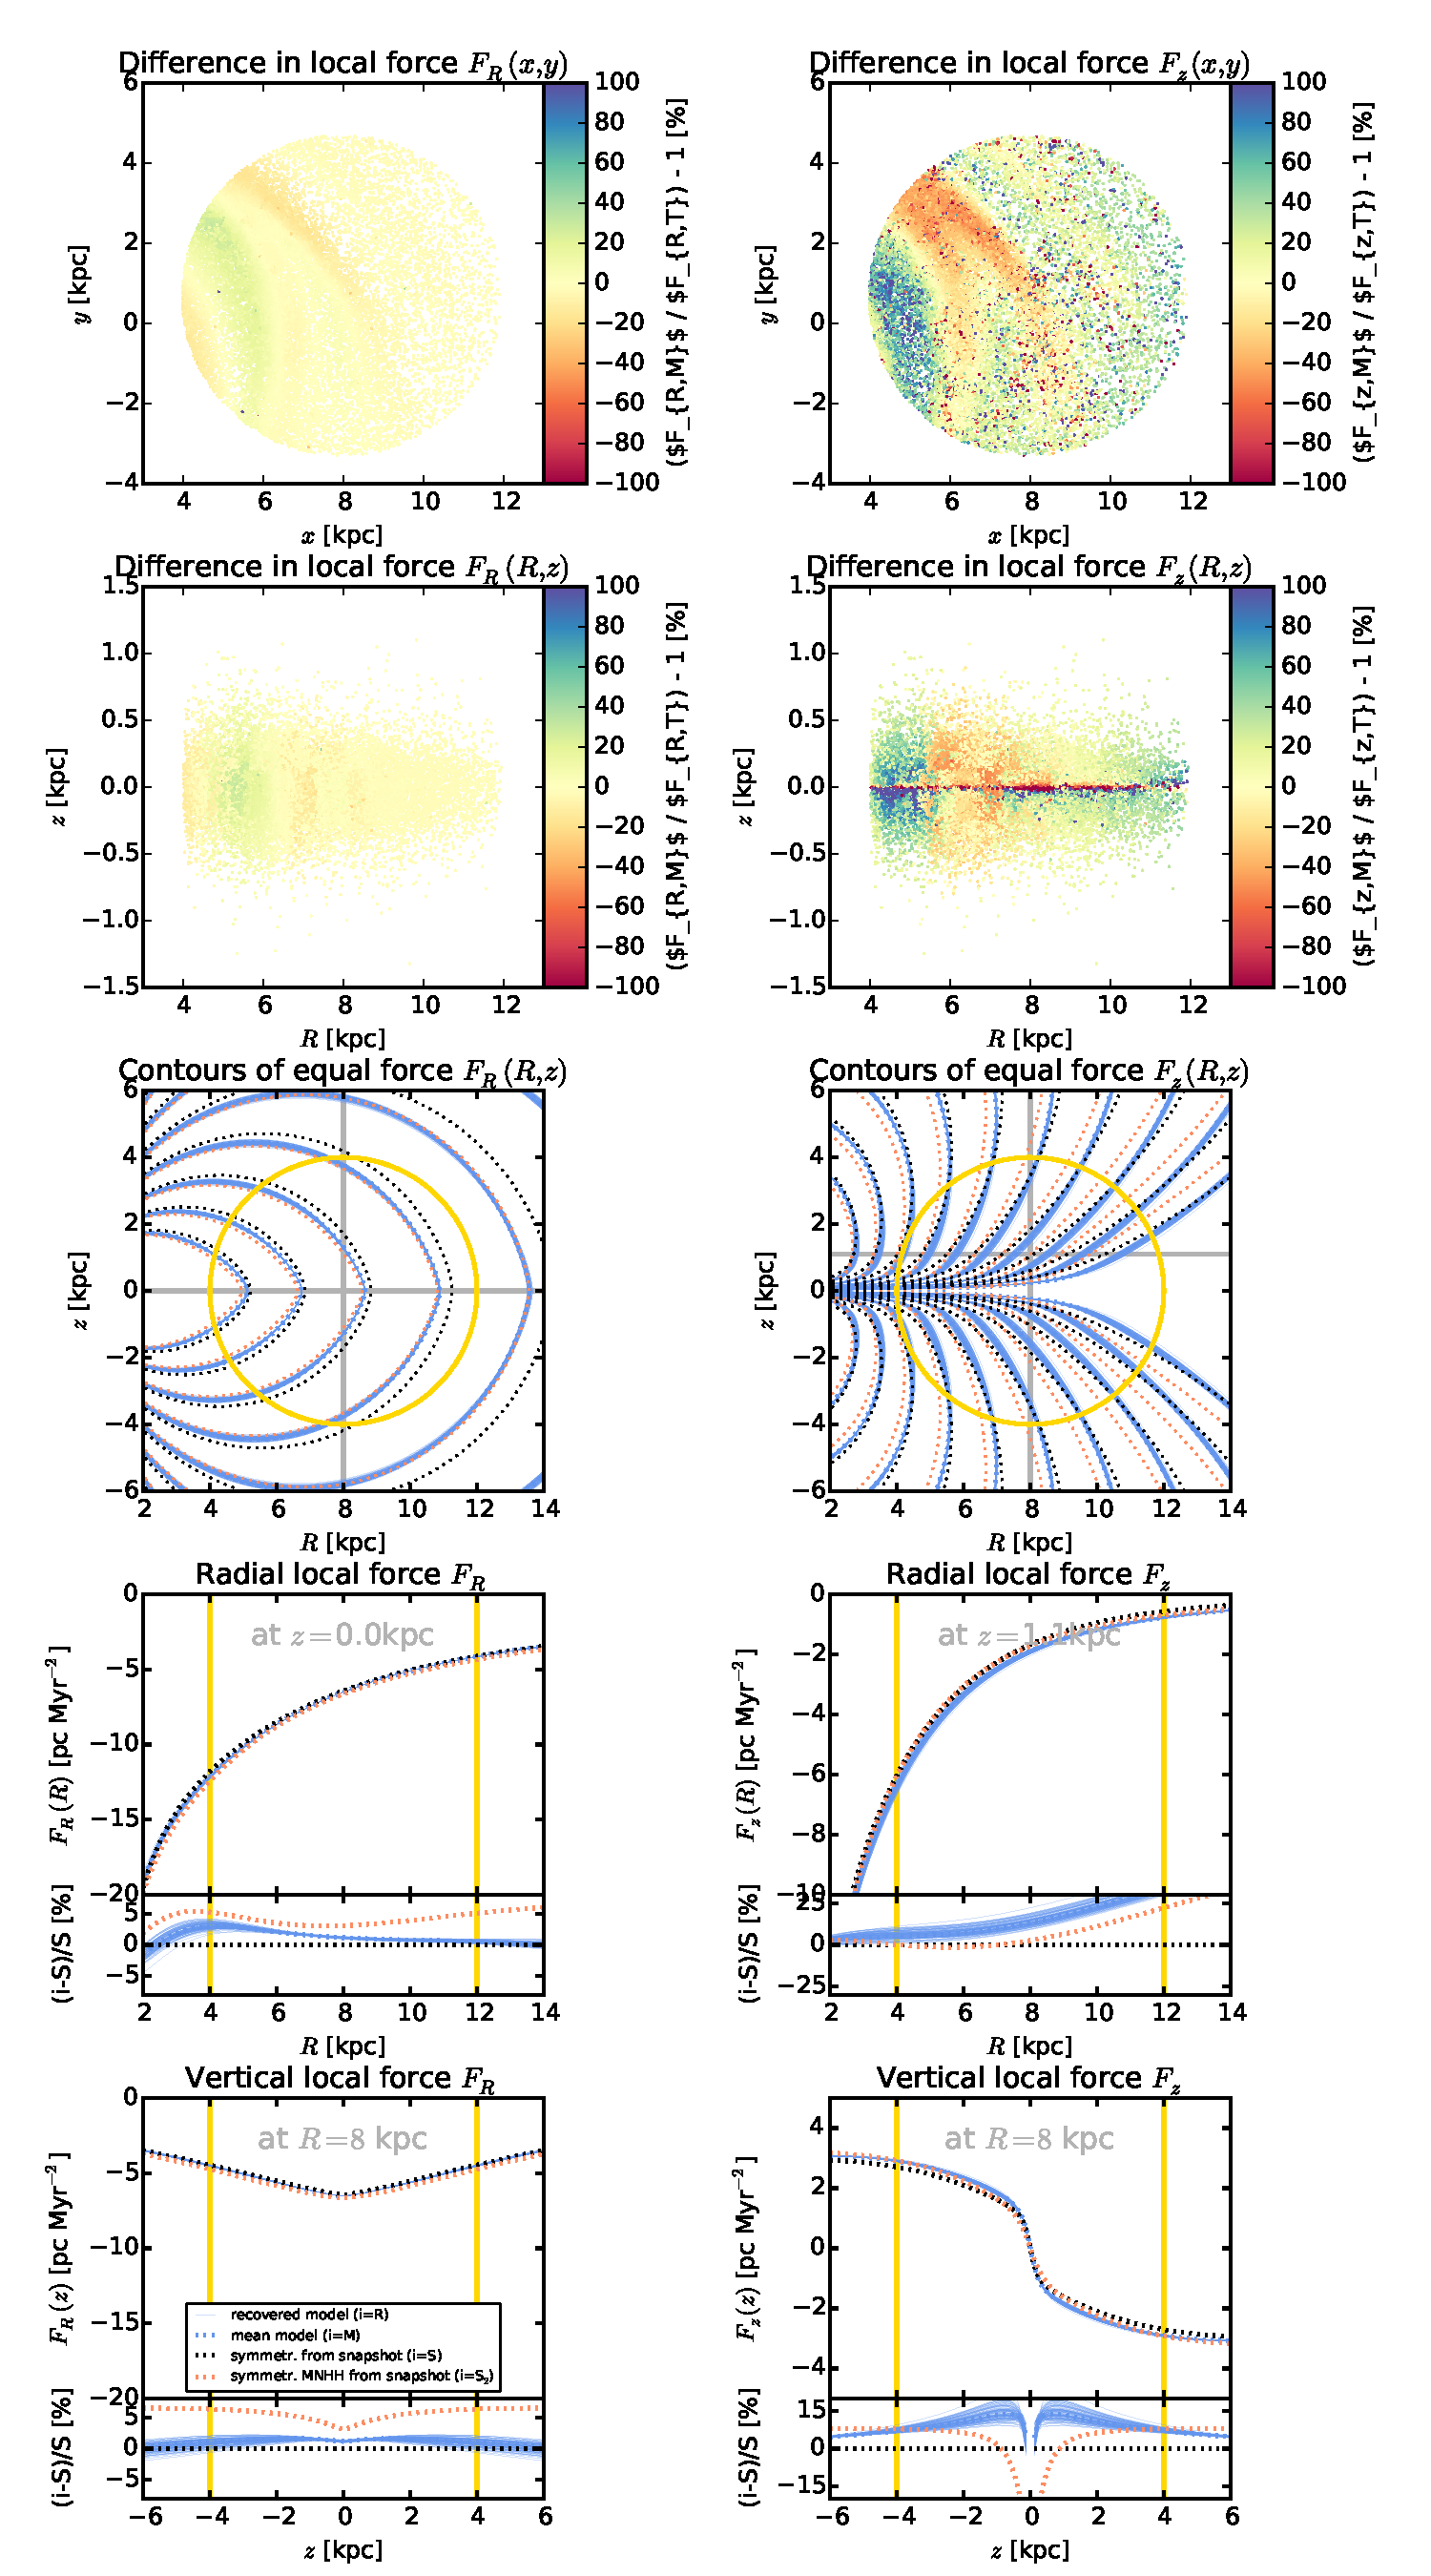
\includegraphics[height=0.9\textheight]{fig/MNdHHdiffSph2_4kpc8Spiral_a_test1_forces_overview_4.pdf}
\caption{Comparison of radial and vertical forces  $F_R=-\partial \Phi / \partial R$ and $F_z = -\partial \Phi / \partial z$ of the true (upper two rows) or symmetrized (lower three rows, black and orange dotted lines) potential of the galaxy simulation snapshot with the potential model recovered with \RM{} (solid blue lines in lower three rows). The upper two rows show the relative difference between the true potential force at the position of each star that entered the \RM{} analysis, and the recovered potential force. The lower three rows compare contours of equal force and force profiles along lines of constant $R$ and $z$. Overall the radial forces are very well recovered, which is related to the well recovery of the circular velocity curve in Figure \Wilma{???}. There are more problems with the vertical force, which is related to the higher surface densities in spiral arms and lower surface density in inter-arm regions, for which the axisymmetric model can only give a average solution. Also, the potential model is not the optimal model to describe the vertical density profile, which becomes also visible in the recovery of the vertical force close to the plane of the disk. \Wilma{[TO DO: Might be, that I have to re-calculate the forces for some of the stars. Write Test that tests if force >1e10 and then recalculates those forces.]}}
\label{fig:???}
\end{figure*}
%====================


\begin{itemize}
\item Figure: Idea for an additional figure (maybe not so interesting): local potential overview plot, scatter plot of stars color coded according to deviation of true and best fit (maybe also symmetrized) potential. normalize potential such that at solar circle pot=0. Both in \% of true potential and number of sigma away.
\end{itemize}

\subsubsection{Recovering the action distribution}

\begin{itemize}
\item Figure: residuals in action space, comparison of true/symmetrized vs. best fit actions (maybe also true vs. best fit in symmetrized potential), overplot Lz=vcirc*Rg of spiral arms
\end{itemize}

\subsection{Investigation of different aspects}

\subsubsection{Test suite}

%====================
\begin{figure*}[!htbp]
\plotone{fig/MNdHHdiffSph2_violins.pdf}
\caption{\Wilma{TO DO: Preliminary. Add more results. Make sure that the "true" potential parameters are the final version.}}
\label{fig:simulation}
\end{figure*}
%====================

\begin{itemize}
\item $r_{max}=1,2,3,4,5kpc$
\item $N_*=20,000$
\item MNHH potential + KKS potential
\item $R_{obs} =5 and 8 kpc$
\end{itemize}



\subsubsection{Survey volume and choice of potential model}

\begin{itemize}
\item Figure: x-axis: $r_{max}$, y-axis: one panel with mean stellar rms deviation in FR and one with Fz. With different potentials and $r_{max}$.
\end{itemize}

\subsubsection{Influence of spiral arms}

\begin{itemize}
\item Figure: x-axis: $\langle \kappa \rangle$, y-axis: one panel with mean stellar rms deviation in FR and one with Fz. Analyses with same potential but at different positions and sizes within the galaxy.
\item Figure: x-axis: $sigma_\kappa$, y-axis: same as above figure.
\end{itemize}

%====================
\begin{figure*}[!htbp]
\plotone{fig/MNdHHdiffSph2_4kpc8Spiral_a_estimate_spiral_strength.pdf}
\caption{Contrast of the spiral arms in the fiducial survey volume of Section \Wilma{???}. As described in Section \Wilma{???} we quantify the strength of the spiral arm \Wilma{???} using Equation \Wilma{???} \Wilma{[TO DO: redo the plot, not all axes labels are shown.]}}
\label{fig:???}
\end{figure*}
%====================

%====================
\begin{figure*}[!htbp]
\plotone{fig/MNdHHdiffSph2_spiral_strength_test.pdf}
\caption{\Wilma{TO DO: This plot will not be in the final paper, it is just for illustration what I get as results for the strength of the spiral arms in the survey volumes. So far it is not that informative... (At least the left panel is a bit weird.)}}
\label{fig:???}
\end{figure*}
%====================



%-----------------------------------------------------------------------------------------------------------------------------------------------------------------------------
%SUMMARY AND CONCLUSION
%-----------------------------------------------------------------------------------------------------------------------------------------------------------------------------
\section{Summary and conclusion}

\bibliography{references_paper2}{}
\bibliographystyle{aasjournal}



\end{document}